\documentclass{article}  
\usepackage{amsmath}
\usepackage{graphicx}
\usepackage{scrextend}
\usepackage[english]{babel}
\usepackage{blindtext}
\usepackage[margin=1in]{geometry}
\usepackage{setspace}
\renewcommand{\baselinestretch}{1.5}

\title{
CSCE578 Assignment 3 Report
}
\author{Sebastian Martin}
\begin{document}
\maketitle


\begin{addmargin}[4em]{4em}

For this project the main goal was to categorize the Student essays from 2014 into clusters. The method chosen in order to do this was a TF-IDF (term frequency – inverse document frequency) computation on all of the documents to gain insight into the most important terms belonging to each document. To prepare the data for this procedure, all of the stop words, and special symbols were removed from all of the documents to clean it for analysis. \\
After the TF-IDF the data needed to be reduced in order to display it on 2 dimensions on a Cartesian plane. There were two options to complete this, PCA (Principle component analysis), and t-SNE (T-distributed Stochastic Neighbor Embedding). Both of these statistical procedures are commonly used in order to linearly correlate data and make it easier to analyze the data. Both of these options were explored in the completion of this project. PCA and t-SNE had generally the same results based on the distributions, however the clustering on PCA was much more vague and spread out than on t-SNE. Because of this, t-SNE was chosen to complete this project as the clusters ended up being denser, more regular, and more consistent. Following this procedure the data dimensions were reduced from 21946 (total amount of unique words in the documents) into 2. \\
This procedure was followed by a k Means clustering of all the points. In order to complete this a total of 8 clusters were chosen. This number was chosen, because smaller cluster sizes resulted in less accurate data with multiple document types being clustered together when they were as related as they should be in the same cluster. When the number was higher than 8, document clusters started being separated, and this caused the grouping to be vaguer than expected, and generally less understandable. One these 8 clusters have been formed, they were given separate colours to differentiate them from each other. \\
From this point is was possible to see which documents clustered together and how they were related. We are able to see which terms were used most often within the documents of each cluster and how important they are to the cluster. On each of these clusters a convex hull was performed and the area of each shape was taken to determine how dense each of the clusters are. \\
\end{addmargin}

\begin{figure}[!hb]
  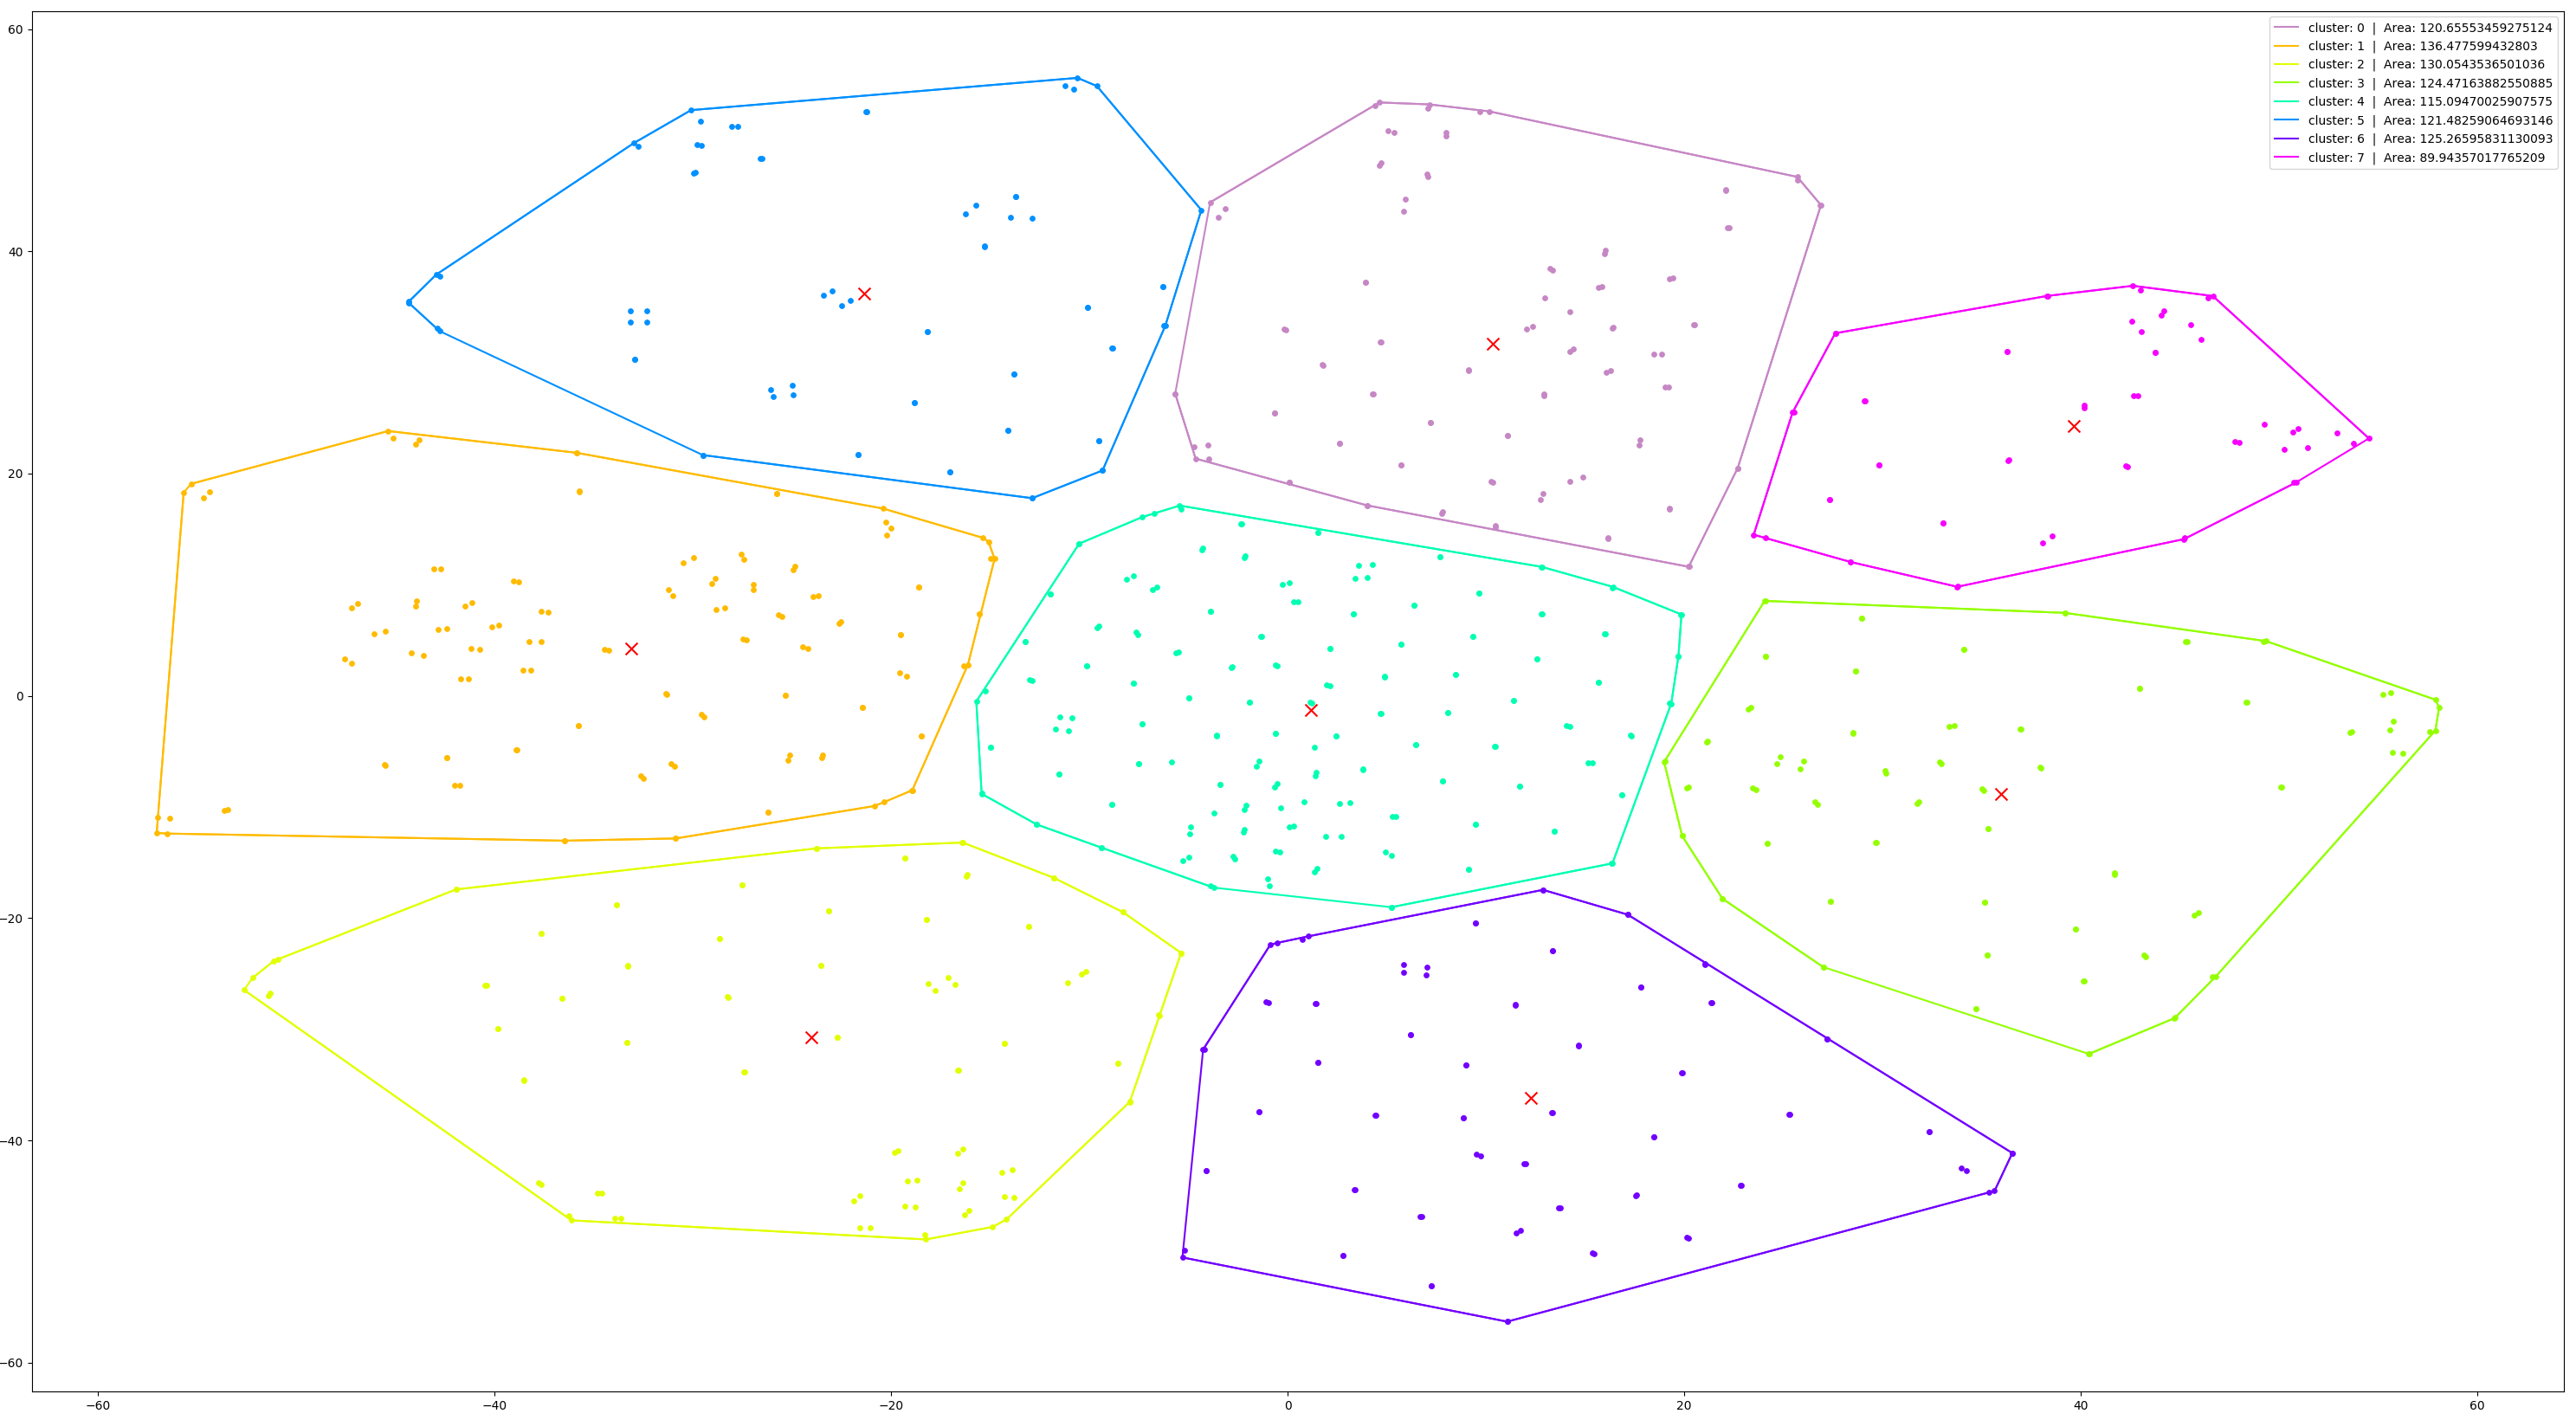
\includegraphics[width=\linewidth]{scatter.png}
  \caption{Scatter plot}
\end{figure}

\begin{figure}[!h]
  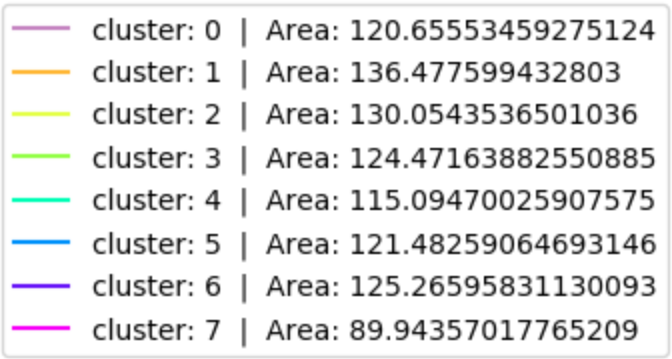
\includegraphics[width=\linewidth]{area.png}
  \caption{Area values}
\end{figure}

\begin{figure}[!h]
  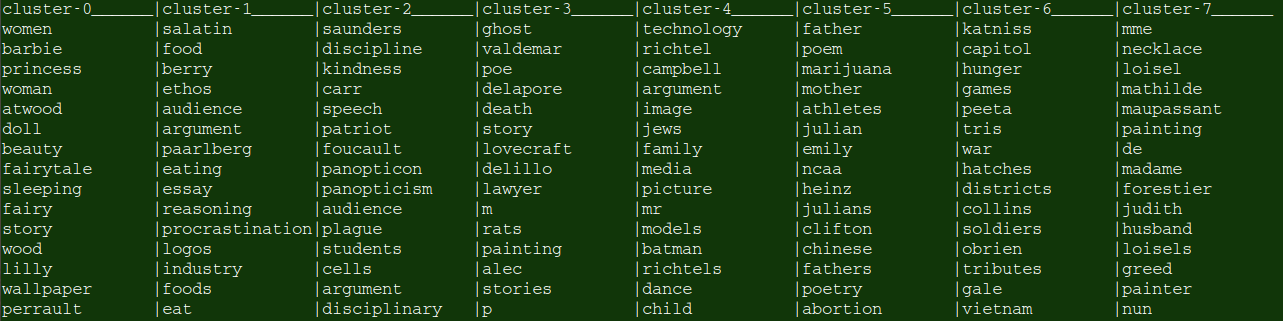
\includegraphics[width=\linewidth]{chart.png}
  \caption{Most common words}
\end{figure}

\begin{addmargin}[4em]{4em}


\end{addmargin}
\begin{addmargin}[4em]{4em}
As can be seen from the data all of the clusters have a decent amount of words that were correlated the closest connection between the words that were easily distinguishable were cluster 0 and  6. This is because they were very general words or very common words in pop culture that can be distinguished by many analyzers. The other words are looser correlated, or have correlations that were not as easily defined by the person analyzing these terms. The most likely cause for this is the fact that the students were given prompts such as artists and their relations between artistic pieces. And looking at the most common terms in each cluster many of the words were names or were generally vague looking to human interpretation.\\
Looking at the areas of each cluster we are able to determine that cluster 7 was the most tightly correlated. The causes for this could be that all of the students who wrote about these subjects used very similar terminology and structures when discussing the subject. Or that not as many students actually wrote about this subject, and because of this there was less variation in the essays that were submitted by them. \\
\\
For a continuation of this project, it would be necessary to determine why each of the documents weighted as they did, and what caused the to be clustered in their positions. Given more time one would have liked to determine the distances between the drafts and the finals of all of the essays in order to get an average distance of the difference of the essays that were written by the students. This would be interesting because just spot checking a few of the clusters one is able to determine that some students had barely any changes to their documents because the points of their essays were virtually in the same spot, however, some of the students had points that has a decent spread and even converged closer to other students essays. If more time was available this would be an interesting process to analyze. \\

\end{addmargin}
Resoures Used:
\begin{addmargin}[4em]{4em}
TF-IDF -Own written code\\
PCA    -SciPy\\
t-SNE  -SciPy\\
kMeans -Scipy\\
Hulls  -SciPy\\
\end{addmargin}


What each file is:
\begin{addmargin}[4em]{4em}
DataAnalysis - The code that completes all of the tasks\\
/data2014/* - The sudent Essays\\
stop.txt - All of the stop words\\
\end{addmargin}




\end{document}
